\chapter{几何形式的Artin互反律}\label{L16}\lecturedate{2020/04/13}\sourcepage{132}
上一讲介绍了几何阿贝尔类域论。回忆，在\lref{L2}和\lref{L3}中，我们已经介绍Artin映射和Artin互反律。本讲讨论Artin互反律的几何形式，并利用Deligne关于Langlands对应的几何构造来证明它。
\section{Artin映射与Artin互反律}\label{L16S1}
先回顾数论情形中的Artin映射和Artin互反律。设$F$为代数数域，$\OO_F$为其代数整数环。设$L/F$为有限Galois扩张，$D$为$\OO_F$在$L$中的整闭包；$\Pp$为$D$中的素理想，位于$\OO_F$的素理想$\p$之上。$\Pp$的分解群为
\[G_{\Pp}=\{\sigma\in\Gal(L/F)\mid\sigma\Pp=\Pp\}.\]
以$L_{\Pp}$、分别$F_{\p}$表示$L$、分别$F$关于素理想$\Pp$、分别$\p$的完备化。则$L_{\Pp}/F_{\p}$也是有限Galois扩张，每个$\sigma\in G_{\Pp}$都诱导$L_{\Pp}$的$F_{\p}$-自同构，因此有映射$i:G_{\Pp}\to\Gal(L_{\Pp}/F_{\p})$。由\eref{命题}{L3S1O2}，它是同构，所以可以将$\Gal(L_{\Pp}/F_{\p})$视为$\Gal(L/F)$的子群。

剩余域$D/\Pp$是$\OO_F/\p$的有限Galois扩张。自然限制映射
\[\Gal(L_{\Pp}/F_{\p})\longrightarrow\Gal((D/\Pp)/(\OO_F/\p))\]
为满射，参见\eref{命题}{L2S2O3}。
\sourcepage{133}
复合映射$G_{\Pp}\xrightarrow{\sim}\Gal(L_{\Pp}/F_{\p})\to\Gal((D/\Pp)/(\OO_F/\p))$的核，称为$\Pp$的\textbf{惯性群}，记为$I_{\Pp}$。若$L_{\Pp}/F_{\p}$非分歧，等价地，$\p$在$L$中非分歧，则$I_{\Pp}=\{1\}$。此时定义$\Pp$处的\textbf{Frobenius元素}为$\Gal((D/\Pp)/(\OO_F/\p))\cong\Gal(\F_{q^f}/\F_q)$中算术Frobenius自同构的唯一原像，记为$\mathrm{Fr}[\Pp]$或$\bigl[\frac{L/F}{\Pp}\bigr]$。

若另选$\p$上方的素理想$\Pp'$，则$G_{\Pp'}$与$G_{\Pp}$共轭，$\mathrm{Fr}[\Pp']$与$\mathrm{Fr}[\Pp]$也共轭。因此以$\mathrm{Fr}[\p]$表示$\mathrm{Fr}[\Pp]$在$\Gal(L/F)$中的共轭类。由于
\[\overline F=\bigcup_{L/F\text{有限Galois}}L,\qquad\Gal(\overline F/F)\cong\varprojlim_{L/F\text{有限Galois}}\Gal(L/F),\]
这些Frobenius共轭类在$\p$非分歧的有限Galois商之间相容，并在相应非分歧商的最大阿贝尔商中给出唯一元素。

设$I_F$为$F$的伊代尔群。将各局部Galois群通过分解群映入整体Galois群，并使用局部互反映射，可定义\textbf{Artin映射}\znote{Artin 映射把伊代尔群映到整体 Galois 群的最大阿贝尔商：在每个素位 $v$ 上取局部互反映射，非分歧处的局部映射就是 $\theta_v(\alpha_v)=\mathrm{Fr}[v]^{v_v(\alpha_v)}$，再把各局部像相乘。它不是某个有限层的映射，而是在所有有限阿贝尔扩张上相容的射有限同态。Artin 互反律断言 $F^\times$ 落在其核中，等价地它经由伊代尔类群分解；整体类域论进一步指出核恰是单位连通分支的闭包，于是「$F$ 的有限阿贝尔扩张」与「伊代尔类群的有限商」一一对应。[来源：J. Neukirch, \textit{Algebraic Number Theory}, Grundlehren der mathematischen Wissenschaften 322，第 VI 章（见第 2 讲参考文献 [N]）。]}
\[\widetilde\theta:I_F\longrightarrow\Gal(\overline F/F)^{\mathrm{ab}},\qquad\widetilde\theta(\alpha)=\prod_v\widetilde\theta_v(\alpha_v).\]
对某个有限扩张中非分歧的有限素位$\p$，其局部映射在该商中满足$\theta_{\p}(\alpha_{\p})=\mathrm{Fr}[\p]^{v_{\p}(\alpha_{\p})}$。有以下Artin互反律\znote{互反律的历史起点是二次互反律，Artin 的版本把「素理想怎样分裂」编码为 Frobenius 共轭类：在每个非分歧素位取局部映射 $\theta_{\p}$，再把各局部像相乘，就得到伊代尔群到整体 Galois 群阿贝尔商的射有限同态。定理断言 $F^\times$（主除子）落在核中，于是 Artin 映射才真正经由伊代尔类群 $I_F/F^\times$ 分解；这条性质是整体类域论主定理的一半，另一半是核恰为单位连通分支的闭包。[来源：nLab 「Artin reciprocity law」，\url{https://ncatlab.org/nlab/show/Artin+reciprocity+law}（Last revised 2024-06-30；2026-11-14 访问）。]}。
\originalnumber{1}
\begin{theorem}[Artin互反律]\label{L16S1O1}
即\eref{定理}{L2S3O7}及\eref{定理}{L3S3O3}：$F^{\times}\subseteq\ker\widetilde\theta$。换言之，
\[\prod_v\theta_v(x)=1,\qquad x\in F^{\times}.\]
\end{theorem}
\section{几何Artin互反律}\label{L16S2}\idx{特征标层}\idx{Lang同源}
设$X$为有限域$\F_q$上的光滑射影几何连通曲线，则函数域$\F_q(X)$为整体域。对每个闭点$x\in X$，其剩余域$k_x$为$\F_q$的有限扩张，因而也是有限域。与数域情形类似，几何情形中有良定义的映射
\[\Gal(\overline{k_x}/k_x)\longrightarrow\Gal(\F_q(X)^{\mathrm{ur}}/\F_q(X))^{\mathrm{ab}}\cong\widehat\pi_1^{\mathrm{ab}}(X).\]
% [Tutor Note: 原书 p135 把该群记作 $\Gal(\overline{\F_{q^n}}/\F_{q^n})$，指的是 $\F_q$-点处的绝对 Galois 群，与 $\Gal(\overline\F_q/\F_q)$ 同义。]
其中$\F_q(X)^{\mathrm{ur}}$为处处非分歧扩张的合成。以$\mathrm{Fr}[x]$表示$\Gal(\overline{k_x}/k_x)$中\textbf{几何Frobenius}的像。
\sourcepage{134}
以$\operatorname{Div}(X)$表示$X$的Weil除子群，则有Artin映射
\[\Psi_X:\operatorname{Div}(X)\longrightarrow\widehat\pi_1^{\mathrm{ab}}(X),\qquad\sum_{j=1}^sa_jx_j\longmapsto\prod_{j=1}^s\mathrm{Fr}[x_j]^{a_j}.\]
Artin互反律的几何形式如下。
\originalnumber{1}
\begin{theorem}\label{L16S2O1}
$\Psi_X$经由有理等价分解，诱导同态$\Psi_X:\operatorname{Pic}_X(\F_q)\to\widehat\pi_1^{\mathrm{ab}}(X)$，并使下图交换：
\begin{figure}[H]\centering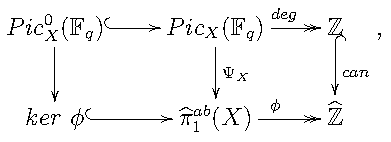
\includegraphics[width=0.3152\paperwidth]{images/L16-p134-reciprocity.pdf}\end{figure}
其中$\phi:\widehat\pi_1^{\mathrm{ab}}(X)\to\widehat{\Z}\cong\widehat\pi_1(\F_q)\cong\Gal(\overline{\F}_q/\F_q)$由结构态射$X\to\Spec\F_q$诱导，参见\eref{定理}{L10S3O2}。这里以几何Frobenius对应于$1$来识别$\Gal(\overline{\F}_q/\F_q)$与$\widehat{\Z}$。
\end{theorem}
我们已经得到以下三类对象之间的一一对应：
\begin{figure}[H]\centering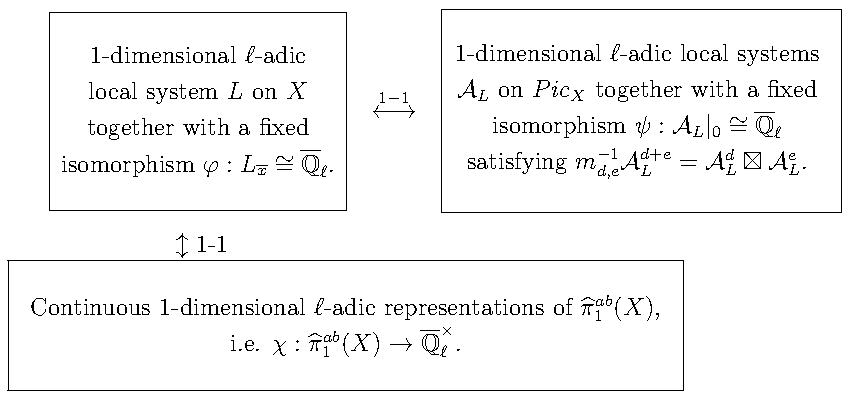
\includegraphics[width=0.6859\paperwidth]{images/L16-p134-three-correspondences.pdf}\end{figure}
为了证明\eref{定理}{L16S2O1}，需要下面的\eref{引理}{L16S2O2}和\eref{引理}{L16S2O3}，它们给出更多一一对应。设$G$为有限域$k$上的连通、分离、有限型交换群概形。
\sourcepage{135}
$G$上的\textbf{$\ell$进特征标层}$\mathcal L$\znoteplain{特征标层可以看成「群同态」的几何版本：一维 $\ell$ 进局部系统给出 $\widehat\pi_1(G)$ 的一维表示；平凡化 $\mathcal L_0\cong\overline\Q_\ell$ 固定单位元处纤维的标架，使「单位元映入 $1$」；乘法同构 $m^{-1}\mathcal L\cong\mathcal L\boxtimes\mathcal L$ 则把群乘法的相容性搬到层上。三者合起来正是「$G$ 上的乘法特征」应有的全部数据，\eref{引理}{L16S2O2}因此能把它们与 $\chi:G(k)\to\overline\Q_\ell^\times$ 一一对应起来；缺少乘法同构时只能得到一般的局部系统。（上下文推断，无外部依据）}，是一个一维$\ell$进局部系统，具有平凡化$\mathcal L_0\cong\overline{\Q}_\ell$及相容的乘法同构$m^{-1}\mathcal L\cong\mathcal L\boxtimes\mathcal L$，其中$m:G\times G\to G$为乘法。
\originalnumber{2}
\begin{lemma}\label{L16S2O2}
下列对象一一对应：
\begin{figure}[H]\centering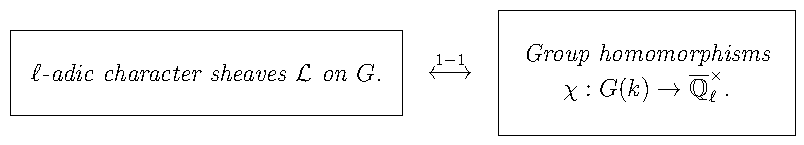
\includegraphics[width=0.6485\paperwidth]{images/L16-p135-Lang-correspondence.pdf}\end{figure}
\end{lemma}
\begin{proof}
先设$\mathcal L$为$G$上的$\ell$进特征标层。对$k$-点$x\in G(k)$，几何Frobenius在纤维$\mathcal L_x$上作用，参见\sref{L12S2}。由于$\mathcal L$为一维，该作用为$\overline{\Q}_\ell^{\times}$中的一个元素。定义
\[\chi:G(k)\longrightarrow\overline{\Q}_\ell^{\times},\qquad x\longmapsto\mathrm{Fr}_x|_{\mathcal L_x}.\]
需要证明$\chi$为群同态。由$m^{-1}\mathcal L\cong\mathcal L\boxtimes\mathcal L$，有$\mathcal L_{x+y}\cong\mathcal L_x\otimes\mathcal L_y$，所以$\chi(x+y)=\chi(x)\chi(y)$。
% [Tutor Note: 原书 p135 此处作 $\mathcal L_{\overline{x+y}}\cong\mathcal L_{\overline x}\otimes\mathcal O_{\overline y}$，其中 $\mathcal O_{\overline y}$ 显系 $\mathcal L_{\overline y}$ 之误（乘法性要求两个因子都是 $\mathcal L$ 的纤维）；译文按正确写法处理。]

反过来，设有群同态$\chi:G(k)\to\overline{\Q}_\ell^{\times}$。由于$k\cong\F_q$，可定义\textbf{Lang同源}\znoteplain{Lang 同源是有限域上特有的构造：$g\mapsto F_q(g)-g$ 把 $G(\overline k)$ 映到自身，并在几何点上成为有限平展覆盖，覆盖变换群恰为 $G(\F_q)$——这就是把「$G(\F_q)$ 的一维表示」与「$G$ 上的局部系统」接起来的桥梁。这里写加号是因为 $G$ 交换；一般群情形用 $g\mapsto F_q(g)g^{-1}$。注意 $F_q$ 是绝对 Frobenius（$g\mapsto g^q$），而不是相对的 $q^n$ 次幂，两者的覆盖变换群不同。（上下文推断，无外部依据）}
\[\varphi:G\longrightarrow G,\qquad g\longmapsto F_q(g)-g,\]
其中$F_q:G\to G$为绝对Frobenius态射$g\mapsto g^q$。Lang同源使$G$成为自身的有限平展Galois覆盖，其覆盖变换群恰为$G(\F_q)$。由平展基本群的定义，有满射$\widehat\pi_1(G)\twoheadrightarrow G(\F_q)$；由于目标交换，它经由$\widehat\pi_1^{\mathrm{ab}}(G)$分解。以几何Frobenius为约定，复合
\[\widehat\pi_1^{\mathrm{ab}}(G)\twoheadrightarrow G(\F_q)\xrightarrow{\chi^{-1}}\overline{\Q}_\ell^{\times}\]
给出一维$\ell$进局部系统$\mathcal L$。

为证明特征标层的乘法性质，只需证明$m^{-1}\mathcal L$和$\mathcal L\boxtimes\mathcal L$的基点纤维作为$\widehat\pi_1(G\times G)$表示同构。分别记两表示为$\rho_m,\rho_\boxtimes$。容易看出它们都经由$\widehat\pi_1(G\times G)\to G(\F_q)\times G(\F_q)$分解，得到下图：
\begin{figure}[H]\centering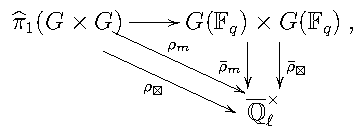
\includegraphics[width=0.2923\paperwidth]{images/L16-p135-characters.pdf}\end{figure}
\sourcepage{136}
其中$\overline\rho_m(g_1,g_2)=\chi(g_1+g_2)^{-1}$，$\overline\rho_\boxtimes(g_1,g_2)=\chi(g_1)^{-1}\chi(g_2)^{-1}$。由于$\chi$为群同态，$\rho_m=\rho_\boxtimes$。可以看出上述两个构造互为逆构造，引理得证。
% [Tutor Note: 原书 p136 此处作 $\overline\rho_m((g_1,g_2))=\chi(g_1+g_2)$、$\overline\rho_\boxtimes((g_1,g_2))=\chi(g_1)\chi(g_2)$，缺指数 $-1$；按本证明中由 $\chi^{-1}$ 构造 $\mathcal L$ 的约定，译文作 $\chi(g_1+g_2)^{-1}$ 与 $\chi(g_1)^{-1}\chi(g_2)^{-1}$。]
\end{proof}
对任意$\F_q$-有理点$x\in X$，一个\textbf{Frobenius作用}就是连续同态$\rho_x:\widehat{\Z}\cong\Gal(\overline{\F}_q/\F_q)\to\overline{\Q}_\ell^{\times}$。设$L$为$X$上的一维局部系统。由\sref{L12S2}，$\Gal(\overline{k_x}/k_x)$作用于纤维$L_{\overline x}$，给出Frobenius作用$\rho_{L,x}:\widehat{\Z}\to\GL(L_{\overline x})\cong\overline{\Q}_\ell^{\times}$。
\originalnumber{3}
\begin{lemma}\label{L16S2O3}
固定$x\in X(\F_q)$。以下两类对象的同构类一一对应：
\begin{figure}[H]\centering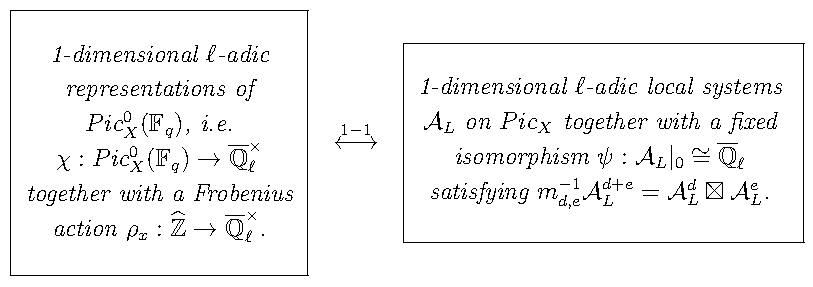
\includegraphics[width=0.6556\paperwidth]{images/L16-p136-Picard-correspondence.pdf}\end{figure}
\end{lemma}
\begin{proof}
从第二类到第一类的映射很直接：取$\mathcal A_L^0$，再应用\eref{引理}{L16S2O2}。Frobenius作用由Deligne定理从$\mathcal A_L$得到的$X$上一维局部系统$L$诱导。

反过来，有同构$m_x^d:\operatorname{Pic}_X^d\to\operatorname{Pic}_X^0$，$\mathcal E\mapsto\mathcal E(-dx)$。Frobenius作用$\rho_x$给出$\{x\}=\Spec\F_q$上的局部系统$L_x$。定义
\[\mathcal A_L^d:=(m_x^d)^{-1}\mathcal A_L^0\otimes L_x^{\otimes d},\]
便得到上述映射的逆构造。
\end{proof}
\begin{proof}[\eref{定理}{L16S2O1}的证明]
先证明下图交换：
\begin{figure}[H]\centering\begin{equation}\tag{2.1}\label{L16eq21}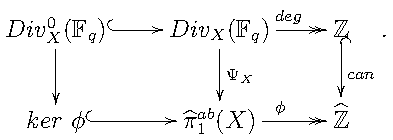
\includegraphics[width=0.3172\paperwidth]{images/L16-p136-divisors.pdf}\end{equation}\end{figure}
\sourcepage{137}
闭点$y:\Spec\F_{q^n}\to X$给出交换三角
\begin{figure}[H]\centering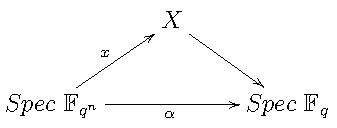
\includegraphics[width=0.2717\paperwidth]{images/L16-p137-closedpoint.pdf}\end{figure}
其中$\alpha$由包含$\F_q\hookrightarrow\F_{q^n}$诱导。因此，$\alpha$诱导的映射
\[\alpha_*:\Gal(\overline{\F}_q/\F_{q^n})\cong\widehat\pi_1(\Spec\F_{q^n})\longrightarrow\widehat\pi_1(\Spec\F_q)\cong\Gal(\overline{\F}_q/\F_q)\]
就是自然包含$\Gal(\overline{\F}_q/\F_{q^n})\hookrightarrow\Gal(\overline{\F}_q/\F_q)$。

另一方面，$\phi\circ\Psi_X(y)=\alpha_*(\mathrm{Fr}_y)$，其中$\mathrm{Fr}_y$为$\Gal(\overline{\F}_q/\F_{q^n})$的几何Frobenius生成元。容易看出，在$\Gal(\overline{\F}_q/\F_q)\cong\widehat{\Z}$的识别下，$\alpha_*(\mathrm{Fr}_y)=\deg y=n$。所以\eqref{L16eq21}中的图交换。

剩下要证明Artin映射$\Psi_X$将主除子映为单位元。正如前面所见，下列四类对象的同构类一一对应：
\begin{figure}[H]\centering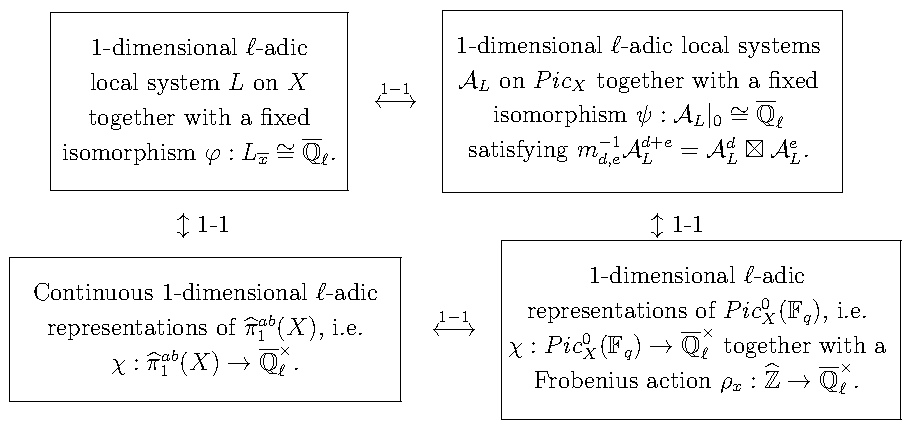
\includegraphics[width=0.7343\paperwidth]{images/L16-p137-four-correspondences.pdf}\end{figure}

由这些对应，每个一维表示$\chi_\pi:\widehat\pi_1(X)\to\overline{\Q}_\ell^{\times}$都确定同态$\chi_P:\operatorname{Pic}_X^0(\F_q)\to\overline{\Q}_\ell^{\times}$及$\rho_x:\Gal(\overline{k_x}/k_x)\to\overline{\Q}_\ell^{\times}$；这里$k_x\cong\F_q$。对任意闭点$y\in X$，我们断言
\begin{equation}\tag{2.2}\label{L16eq22}
\chi_\pi(\mathrm{Fr}[y])=\chi_P\bigl(\OO_X(y-dx)\bigr)\rho_x(\mathrm{Fr}_x)^d,\qquad d=\deg y=[k_y:\F_q].
\end{equation}
\sourcepage{138}
记$x_d$为$x$在$\F_{q^d}$上的基变换。

为证明\eqref{L16eq22}，先注意$\chi_\pi$给出$X$上的一维$\ell$进局部系统$L$。$\Gal(\overline{k_y}/k_y)$在$L_{\overline y}$上的作用诱导$\rho_y:\Gal(\overline{k_y}/k_y)\to\GL(L_{\overline y})$，得到以下交换三角：
\begin{figure}[H]\centering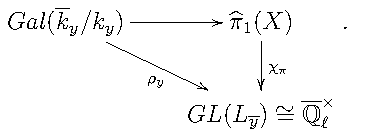
\includegraphics[width=0.2949\paperwidth]{images/L16-p138-monodromy.pdf}\end{figure}
另一方面，$\chi_P$给出$\operatorname{Pic}_X^0$上的$\ell$进特征标层$\mathcal A_L^0$。记$\widetilde y$为$y$在$\F_{q^d}$上的一个提升（即$\widetilde y:\Spec\F_{q^d}\to X$的像为闭点$y$），因而$\OO_X(\widetilde y)$为$\operatorname{Pic}_X^1$的$\F_{q^d}$-点。按\eref{引理}{L16S2O3}的构造，$\operatorname{Pic}_X^1$上的一维局部系统满足
\[\mathcal A_L^1=(m_x^1)^{-1}\mathcal A_L^0\otimes L_x.\]
由于$x_d$为位于$x$上方的$\F_{q^d}$-点，$\OO_X(\widetilde y-x_d)$为$\operatorname{Pic}_X^0$的$\F_{q^d}$-点。由Lang构造，其几何Frobenius在$\mathcal A_L^0$该纤维上的作用为
\[\chi_P\bigl(N_{\F_{q^d}/\F_q}\OO_X(\widetilde y-x_d)\bigr)=\chi_P(\OO_X(y-dx)),\]
因此，几何Frobenius在$(\mathcal A_L^1)_{\OO_X(\widetilde y)}$上的作用为$\chi_P(\OO_X(y-dx))\rho_x(\mathrm{Fr}_{x_d})$。由Deligne定理，$AJ_1^{-1}\mathcal A_L^1\cong L$，从而有交换图：
\begin{figure}[H]\centering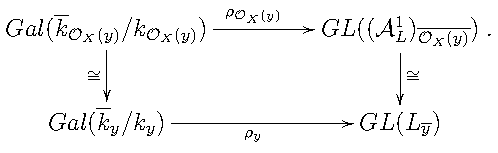
\includegraphics[width=0.4014\paperwidth]{images/L16-p138-comparison.pdf}\end{figure}
通过自然包含$\Gal(\overline{k_{x_d}}/k_{x_d})\hookrightarrow\Gal(\overline{k_x}/k_x)$，有$\mathrm{Fr}_{x_d}=(\mathrm{Fr}_x)^d$，于是得到\eqref{L16eq22}。

因此，对任意主除子$D$及$\widehat\pi_1(X)$的任意一维表示$\chi$，均有$\chi\circ\Psi_X(D)=1$。

因为$\widehat\pi_1(X)$为射有限群，对任意$1\ne s\in\widehat\pi_1(X)$，均有有限商$q_s:\widehat\pi_1(X)\to G_s$使$q_s(s)\ne1$。若$s$在$\widehat\pi_1^{\mathrm{ab}}(X)$中的像非平凡，还可取$G_s$为交换群。由有限阿贝尔群表示论的基本事实，可以找到特征标$\chi_s:G_s\to\overline{\Q}_\ell^{\times}$，使$\chi_s(q_s(s))\ne1$。复合$\chi_s\circ q_s$便是一个在$s$处非平凡的一维表示。所以，对所有主除子$D$，必有$\Psi_X(D)=1$。
\end{proof}
\sourcepage{139}
\needspace{5\baselineskip}\section{第16讲参考文献}\label{L16S3}
\begin{references}
\refitem{L16bibT}{T} Péter Tóth, \emph{Geometric abelian class field theory}, Thesis for MD at Univ. Utrecht, available at \url{http://math.bu.edu/people/magner/Seminar/GCFTthesis.pdf}.
\end{references}
